\section{Introduction} \label{sec:intro}

\begin{figure*}
	\centering
	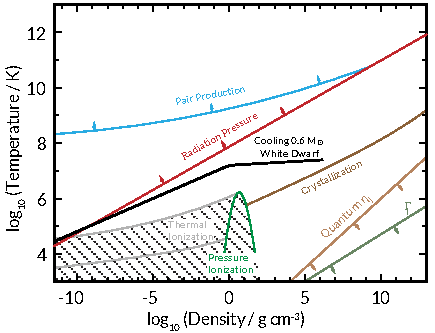
\includegraphics[width=0.9\textwidth]{skye_eos_no_labels.pdf}
	\caption{Coverage of the Skye EOS in the ($\rho,T$) plane. Shown is approximately where radiation pressure (red) 
                 dominates the gas pressure, thermodynamics from $e^-e^+$ pair production (light blue) dominates, crystallization
                 of ions (brown) begins, thermal (light gray) and pressure (green) ionization of atoms occurs.
%                 Regions where degeneracy (defined by $\mu_e/kT$, where $\mu_e$ is the electron chemical potential) 
%                 and special relativity (defined by $kT/m_ec^2$) are dominant are labeled (dark gray).
                 Lines of constant ion quantum parameter $\eta_j$ (light brown)
                 and ion interaction strength $\Gamma_j$ (dark green) are indicated in the lower-right, and attached arrows denote directions of increasing $\eta_j$ and $\Gamma_j$.
                 The dotted region marks where Skye's assumption of full ionization is a poor approximation.
                 An example profile, from core to surface, of a cooling white dwarf (black) is illustrated.}
	\label{fig:skye_eos}
\end{figure*}

The equation of state (EOS) of ionized matter is a key ingredient in models of stars, gas giant planets, accretion disks, and many other astrophysical systems.
These applications span many orders of magnitude in both density and temperature, and include both low-density systems that are thermally ionized (e.g., stellar atmospheres) and high-density ones that are pressure-ionized (e.g., planetary interiors).
Moreover matter can have many different compositions, ranging from pure hydrogen to exotic mixtures of heavy metals.
As a result, approximations to nature's EOS of ionized matter must capture a wide variety of physics (Figure~\ref{fig:skye_eos}) including relativity, quantum mechanics, electron degeneracy, pair production, phase transitions, and chemical mixtures.

Despite these challenges, several different equations of state have been introduced for ionized matter
\citep[e.g.,][]{1961ApJ...134..669S,eggleton_1973_aa,bludman_1977_aa,daeppen_1990_aa,pols_1995_aa,rogers_1996_aa,blinnikov_1996_aa,timmes_1999_aa,gong_2001_ab,dappen_2010_aa}.
\citet{1990JPhys..51.1607C} introduced an EOS for non-relativistic ionized hydrogen, incorporating sophisticated quantum and electron screening corrections.
Improvements then led to the PC EOS~\citep{CP1998,PhysRevE.62.8554,2009PhRvE..80d7401P,Potekhin2010}.
PC allows for arbitrary compositions and incorporates relativistic ideal electrons as well as modern prescriptions for electron screening and multi-component plasmas.
\citet{2013A&A...550A..43P} extended the PC EOS to include the effects of strong magnetic fields such as those found in neutron stars.
One of the distinguishing features of the PC EOS is the use of analytic prescriptions to capture non-ideal physics.

One of the limitations of the PC EOS is that it does not capture the effects of electron-positron pair production at high temperatures, which is important for the pair instability in massive stars~\citep{1967ApJ...148..803R}.
The treatment of electron degeneracy and the ideal quantum electron gas is also approximate, based on fitting formulas which approximate the relevant Fermi integrals.
These limitations are addressed by the HELM EOS~\citep{Timmes2000}.
While HELM does not include the sophisticated non-ideal corrections which are a defining strength of PC, it provides a tabulated Helmholtz free energy treatment of an ideal quantum electron-positron plasma, obtained by high-precision evaluation of the relevant Fermi-Dirac integrals \citep{cloutman_1989_aa,aparicio_1998_aa,gong_2001_aa}.
As such, HELM accurately and efficiently handles relativistic effects, degeneracy effects, and high-temperature pair production.

In this article we build on this progress by presenting a new equation of state, \skye, an EOS designed to handle density and temperature inputs over the range $10^{-12}\,\mathrm{g\,cm^{-3}} < \rho < 10^{13}\,\mathrm{g\,cm^{3}}$ and $10^3\,\mathrm{K} < T < 10^{13}\,\mathrm{K}$ (Figure~\ref{fig:skye_eos}).
\skye \ assumes material is fully-ionized, so the suitability
of the result is subject to the (composition-dependent) constraint that material is either pressure-ionized ($\rho \gtrsim 10^3\,\mathrm{g\,cm^{-3}}$) or thermally-ionized ($T \gtrsim 10^{5}\,\mathrm{K}$)\footnote{See Section~\ref{sec:limitations} for detailed composition-dependent ionization limits.}.
Further limits to Skye's suitability can arise due to violations of its other physics assumptions.
Building on HELM, we use the full ideal equation of state for electrons and positrons, accounting for degeneracy and relativity.
Ions are assumed to be a classical ideal gas.
We then add non-ideal classical and quantum corrections to account for electron-electron, electron-ion, and ion-ion interactions following a multi-component ion plasma prescription.
These corrections are generally similar to those used by the PC EOS, though we have used updated physics prescriptions in some instances~\citep[e.g., those of][]{2019MNRAS.488.5042B}.

Thermodynamic quantities in \skye\ are derived from a Helmholtz free energy to ensure thermodynamic consistency.
Automatic differentiation machinery allows extraction of arbitrary derivatives from an analytic Helmholtz free energy, allowing \skye\ to provide the high-order derivatives needed for stellar evolution calculations~\citep[e.g.,][]{Paxton2011}.
We further leverage this machinery to make the EOS easily extensible: adding new or refined physics to \skye\ is as easy as writing a formula for the additional Helmholtz free energy. The often painstaking and error-prone process of taking and programming analytic first, second, and even third derivatives of the Helmholtz free energy is eliminated. 
In this way \skye\ is a \emph{framework} for rapidly developing and prototyping new EOS physics as advances are made in numerical simulations and analytic calculations. We emphasize that \skye\ is not tied to a specific set of physics choices; \skye\ in 10 years is unlikely to be the same as \skye\ as described in this article.

In addition to being a single EOS which can be used at both high temperatures, like HELM, and high densities, like PC, \skye\ currently includes two significant physical improvements.
First, whereas PC fixes the location of Coulomb crystallization of the ions, \skye\ picks between the liquid and solid phase to minimize the Helmholtz free energy.
This enables a self-consistent treatment of the phase transition, albeit one currently without chemical phase separation, and means that the Helmholtz free energy is continuous across the transition.
Secondly, we introduce the technique of \emph{thermodynamic extrapolation}, 
which provides a principled way to extend Helmholtz free energy fitting formulas beyond their original range of applicability
and thus enables comparisons of the liquid and solid phase Helmholtz free energies.

This paper is structured as follows.
Important symbols are defined in Table~\ref{tab:symbols}.
In Section~\ref{sec:free} we explain the various terms which contribute to the Helmholtz free energy in \skye, as well as the new handling of phase transitions (Section~\ref{sec:non-ideal}) and thermodynamic extrapolation (Section~\ref{sec:extrapolate}).
Section~\ref{sec:thermo} shows how we extract thermodynamic quantities from the Helmholtz free energy.
We also introduce auxiliary quantities which allow stellar evolution software instruments to incorporate the latent heat of the Coulomb crystallization in a smooth manner.
Section~\ref{sec:limitations} discusses some of the current physics limitations of \skye,
which is principally that it does not extend to cases of partially ionized or neutral matter, or dense nuclear matter \citep{hempel_2012_aa}.
Section~\ref{sec:autodiff} introduces our automatic differentiation machinery.
In Section~\ref{sec:examples} we compare \skye\ to the PC and HELM equations of state and evaluate the quality of derivatives and thermodynamic consistency in \skye.
We also calculate white dwarf cooling tracks and demonstrate that \skye\ properly accounts for the latent heat of crystallization
(Section~\ref{sec:cooling}).
In Section~\ref{sec:speed} we demonstrate that \skye\ has comparable runtime performance to PC, making it viable for use in stellar evolution calculations.
\skye\ is open source and open-knowledge, and Section~\ref{sec:avail} describes options for obtaining and using \skye.
We conclude with a discussion of future work in Section~\ref{sec:conc}.

\startlongtable
\begin{deluxetable}{llr}
  \tablecolumns{3}
  \tablewidth{0.5\textwidth}
  \tablecaption{Important symbols.\label{tab:symbols}}
  \tablehead{\colhead{Name} & \colhead{Description} & \colhead{Appears}}
  \startdata
$T$ & Temperature & \ref{sec:intro}\\
$\rho$ & Density & \ref{sec:intro}\\
$F$ & Helmholtz Free Energy & \ref{sec:free}\\
$F_{\rm ideal}$ & Ideal Free Energy & \ref{sec:free}\\
$F_{\textrm{non-ideal}}$ & Non-ideal Free Energy & \ref{sec:free}\\
$F_{\rm rad}$ & Radiation Gas Free Energy & \ref{sec:ideal}\\
$F_{\rm ideal \ e^- e^+}$ & Ideal Electron-Positron Free Energy & \ref{sec:ideal}\\
$F_{\rm ideal \ ion}$ & Ideal Ion Free Energy & \ref{sec:ideal}\\
$F_{\rm ideal \ mix}$ & Ideal Ion Mixing Free Energy & \ref{sec:ideal}\\
$a$ & Radiation Gas Constant & \ref{sec:ideal}\\
$k_{\rm B}$ & Boltzmann Constant & \ref{sec:ideal}\\
$m_j$ & Mass of species $j$ & \ref{sec:ideal}\\
$y_j$ & Number fraction of ion species $j$ & \ref{sec:ideal}\\
$\bar{m}$ & Average ion mass & \ref{sec:ideal}\\
$n_j$ & Number density of species $j$ & \ref{sec:ideal}\\
$n_{Q,j}$ & Quantum density of ion species $j$ & \ref{sec:ideal}\\
$M_{\rm spin}$ & Spin multiplicity of ion species $j$ & \ref{sec:ideal}\\
$\hbar$ & Reduced Planck Constant & \ref{sec:ideal}\\
$a_j$ & Sphere radius of species $j$ & \ref{sec:non-ideal}\\
        & $(3n_j/4\pi)^{-1/3}$&\\
$r_{s,j}$ & Non-dimensional radius of species $j$ & \ref{sec:non-ideal}\\
        &$Z_j^2 m_j e_j^2 a_j / \hbar^2$&\\
$Z_j$ & Charge of species $j$  & \ref{sec:non-ideal}\\
        &($-1$ for electrons)&\\
$\Gamma_j$ & Coupling parameter of species $j$ & \ref{sec:non-ideal}\\
        &$Z_j^2 e^2 / a_j k_{\rm B} T$&\\
$\eta_j$ & Quantum Parameter of species $j$ & \ref{sec:non-ideal}\\
        &$(\hbar/k_{\rm B} T)\sqrt{4\pi e^2 n_j Z_j^2/m_j}$&\\
$p_{\rm F}$ & Fermi Momentum & \ref{sec:non-ideal}\\
$x_r$ & Relativity Parameter $p_{\rm F}/m_e c$ & \ref{sec:non-ideal}\\
$\gamma$ & Fermi Lorentz Factor & \ref{sec:non-ideal}\\
        & $\sqrt{1+x_r^2}$&\\
$E_{\rm F}^{\rm NR}$ & Non-relativistic Fermi Energy & \ref{sec:non-ideal}\\
$h(\alpha)$ & Switch function & \ref{sec:non-ideal}\\
$\alpha$ & Switch parameter & \ref{sec:non-ideal}\\
        &$3 k_{\rm B} T \gamma / 2 E_{\rm F}^{\rm NR}$&\\
$e$ & Specific internal energy & \ref{sec:extrapolate}\\
$s$ & Specific entropy & \ref{sec:extrapolate}\\
$T_{\rm b}$ & Extrapolation Temperature & \ref{sec:extrapolate}\\
$\Gamma_{\rm max}^{\rm liquid}$ & Liquid extrapolation $\Gamma_j$& \ref{sec:extrapolate}\\
$\Gamma_{\rm min}^{\rm solid}$ & Solid extrapolation $\Gamma_j$& \ref{sec:extrapolate}\\
$p$ & Pressure & \ref{sec:thermo}\\
$c_v$ & Specific heat at constant volume & \ref{sec:thermo}\\
$c_p$ & Specific heat at constant pressure & \ref{sec:thermo}\\
$\chi_T$ & Thermal susceptibility & \ref{sec:thermo}\\
$\chi_\rho$ & Density susceptibility & \ref{sec:thermo}\\
$\Gamma_1$ & First adiabatic exponent & \ref{sec:thermo}\\
$\Gamma_2$ & Second adiabatic exponent & \ref{sec:thermo}\\
$\Gamma_3$ & Third adiabatic exponent & \ref{sec:thermo}\\
$\nabla_{\rm ad}$ & Adiabatic Gradient & \ref{sec:thermo}\\
$c_s$ & Sound speed & \ref{sec:thermo}\\
$\phi$ & Smoothed phase parameter & \ref{sec:thermo}\\
$L_T$ & Latent $T ds/d\ln T$ & \ref{sec:thermo}\\
$L_\rho$ & Latent $T ds/d\ln \rho$ & \ref{sec:thermo}\\
$T_{j}^{\rm ion}$ & Full-ionization $T$ of species $j$ & \ref{sec:limitations}\\
$\rho_{j}^{\rm ion}$ & Full-ionization $\rho$ of species $j$ & \ref{sec:limitations}\\
$\rho_{j,\rm nuclear}$ & Nuclear density of species $j$ & \ref{sec:limitations}\\
$T_{\rm QCD}$ & Temperature of & \ref{sec:limitations}\\
 & proton rest mass-energy & \\
  \enddata
\end{deluxetable}


